\documentclass{beamer}

\usetheme{Madrid}

\usepackage{lipsum}
\usepackage{multicol}
\usepackage{listings}
\usepackage{multirow}

% Define a custom color
\definecolor{backcolour}{rgb}{255,255,255}
\definecolor{codegreen}{rgb}{0,0.6,0}

% Define a custom style
\lstdefinestyle{myStyle}{
    backgroundcolor = \color{backcolour},   
    commentstyle = \color{codegreen},
    basicstyle=\linespread{0.4}\tiny,
    breakatwhitespace=false,         
    breaklines=true,        
    keepspaces=true,                               
    showspaces=false,                
    showstringspaces=false,
    showtabs=false,                  
    tabsize=2,
}

% Use \lstset to make myStyle the global default
\lstset{style=myStyle}

\usepackage{graphicx}
\usepackage{listings}
\usepackage{verbatim}
\linespread{1.5}
\usepackage{pgfplots}
\usepackage{tikz}

\usepackage{amsmath, amsthm, amssymb, latexsym}

%\newtheorem{definition}{Definition}

\newcommand{\pathtoimages}{/Users/charlesrambo/Desktop/Bootcamp24/Images}

\title{Unit 4: Covariance Matrices, PCA, and Stochastic Calculus}
\author{Charles Rambo}
\institute{UCLA Anderson}
\date{2024}


\begin{document}
\input{systempreamble}


\frame{\titlepage}

\begin{frame}[allowframebreaks]

\frametitle{Table of Contents}
\tableofcontents
\end{frame}


\section{Covariance Matrices}

\begin{frame}
\begin{center}
\Huge Covariance Matrices
\end{center}
\end{frame}

\begin{frame}
\frametitle{Covariance Matrix}
\small
\begin{Definition}
Suppose ${\boldsymbol X} = \left(X_1, X_2,\ldots, X_n\right)^T$ is a multivariate random variable, and ${\boldsymbol \mu} = (\mu_1, \mu_2,\ldots,\mu_n)^T$. The {\bf covariance matrix} of $X$ is
$$
\Sigma = E\left[({\boldsymbol X} - {\boldsymbol \mu}) ({\boldsymbol X} - {\boldsymbol \mu})^T\right].
$$
\end{Definition}
Notice that
$$
\Sigma_{ij} = \begin{cases} \text{Var}(X_i),	& i = j\\ \text{Cov}(X_i, X_j),	&	i\neq j.\end{cases}
$$
\end{frame}

\begin{frame}
\frametitle{Multivariate Normal Distribution}
\begin{Definition}
The {\bf multivariate normal distribution} or {\bf Gau\ss ian distribution} of dimension $k$ has probability density function
$$
f({\boldsymbol x}) = \frac{1}{\sqrt{ (2\pi)^k |\Sigma|}} \text{exp}\left(-\frac{1}{2}\left({\boldsymbol x} - {\boldsymbol \mu}\right)^T\Sigma^{-1}({\boldsymbol x} - {\boldsymbol \mu})\right),
$$
where $ {\boldsymbol \mu}$ is in $\mathbb{R}^k$ and $\Sigma$ is the distribution's $k\times k$ covariance matrix. To denote that $ {\boldsymbol X}$ follows a multivariate normal distribution, we write $ {\boldsymbol X}\sim{\mathcal{N}( {\boldsymbol \mu}, \Sigma)}$ or $ {\boldsymbol X}\sim{\mathcal{N}_k({\boldsymbol \mu}, \Sigma)}$ .
\end{Definition}

\end{frame}

\begin{frame}
\frametitle{Bivariate Normal Distribution Python Example}
\small
\begin{Example}
Sample 100 points from $\mathcal{N}\left( {\boldsymbol \mu}, \Sigma\right)$, where $ {\boldsymbol \mu} = (0, 0)^T$ and $\Sigma = $
\begin{multicols}{2}
\begin{enumerate}
\item[(a)] $\left(\begin{array}{c c} 1	&	0\\ 0	&	1\end{array}\right)$
\item[(b)] $\left(\begin{array}{c c} 1	&	0.5\\ 0.5	&	1\end{array}\right)$
\item[(c)] $\left(\begin{array}{c c} 1	&	-0.5\\ -0.5	&	1\end{array}\right)$
\item[(d)] $\left(\begin{array}{c c} 1	&	1\\ 1	&	1\end{array}\right)$.
\end{enumerate}
\end{multicols}
Graph the results.
\end{Example}


\end{frame}

\begin{frame}[fragile]
\frametitle{Bivariate Normal Distribution Example}
\begin{multicols}{2}
\begin{lstlisting}[language=Python]
# Import modules
import numpy as np
import matplotlib.pyplot as plt
from scipy.stats import multivariate_normal

# Use LaTeX
plt.rcParams['text.usetex'] = True

# Use Seaborn style
plt.style.use('seaborn')

# Set random seed
np.random.seed(0)

# Create list for problem parts
parts = ['a', 'b', 'c', 'd']

# Create list of covariance matrices
covs = [np.array([[1, 0], 
					[0, 1]]), 
        	np.array([[1, 0.5], 
					[0.5, 1]]), 
        	np.array([[1, -0.5], 
					[-0.5, 1]]), 
        	np.array([[1, 1], 
					[1, 1]])]

# Set up subplots
fig, ax = plt.subplots(2, 2, sharex = True, sharey = True, figsize = (10, 7))

# Loop over titles and covariance matrices 
for i, part, cov in zip(range(4), parts, covs):
    
    # Get the row and column
    row, col = i // 2, i%2

    # Generate values
    vals = multivariate_normal.rvs(mean = np.zeros(2), cov = cov, size = 100)
    
    # Get x- and y-coordinates
    x, y = zip(*vals)
    
    # Plot the values
    ax[row, col].scatter(x, y)
    
    # Get title
    title = part + r': $\rho$ = ' + str(cov[0, 1])
    
    # Give the plot a title
    ax[row, col].title.set_text(title)

# Give entire figure title
fig.suptitle('Bivariate Normals')

# Save the figure
plt.savefig(path + r'ex4-1.png')

plt.show()
\end{lstlisting}
\end{multicols}
\end{frame}

\begin{frame}
\frametitle{Bivariate Normal Distribution Example Result}
\begin{figure}
\centering
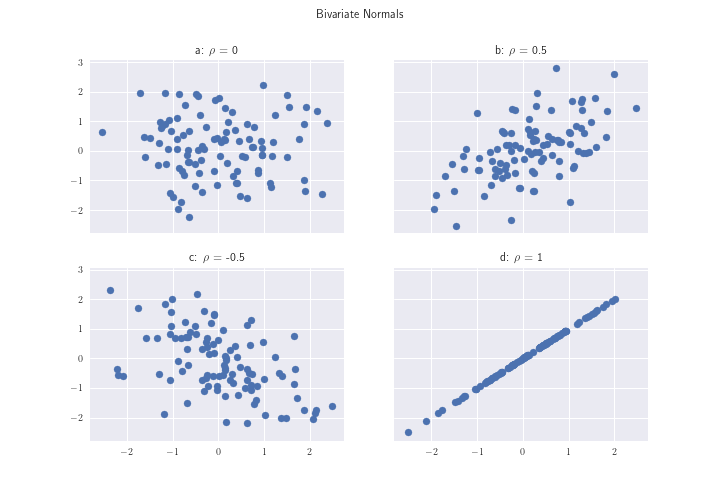
\includegraphics[scale = 0.4]{\pathtoimages/ex4-1.png}
\end{figure}
\end{frame}


\begin{frame}
\frametitle{Sample Covariance}
In the sample covariance matrix, we divide by $n-1$ instead of $n$. Using the \texttt{pandas} data frame \texttt{df} the sample covariance matrix would be  \texttt{df.cov()}.

\end{frame}

\begin{frame}[fragile]
\frametitle{Sample Covariance Matrix Example}
\small 
Here is some code to get the sample covariance matrix for the {\it current} S\&P constituents. The uploaded data are the daily constituents' returns from January 1, 2019 to May 31, 2024 which are available over the whole time range. The data source is {\it Yahoo! Finance}. Check out the Unit 4 Code Snippets to see how the data were extracted.
\begin{lstlisting}[language=Python]
# Import modules
import pandas as pd

# Load in data; make date the index
data = pd.read_csv(data_path, index_col = 'Date')

# Get covariance matrix
S = data.cov()

S
\end{lstlisting}


\end{frame}

\begin{frame}
\frametitle{Sample Covariance Matrix Result}
The output looks like this:
\begin{figure}
\centering
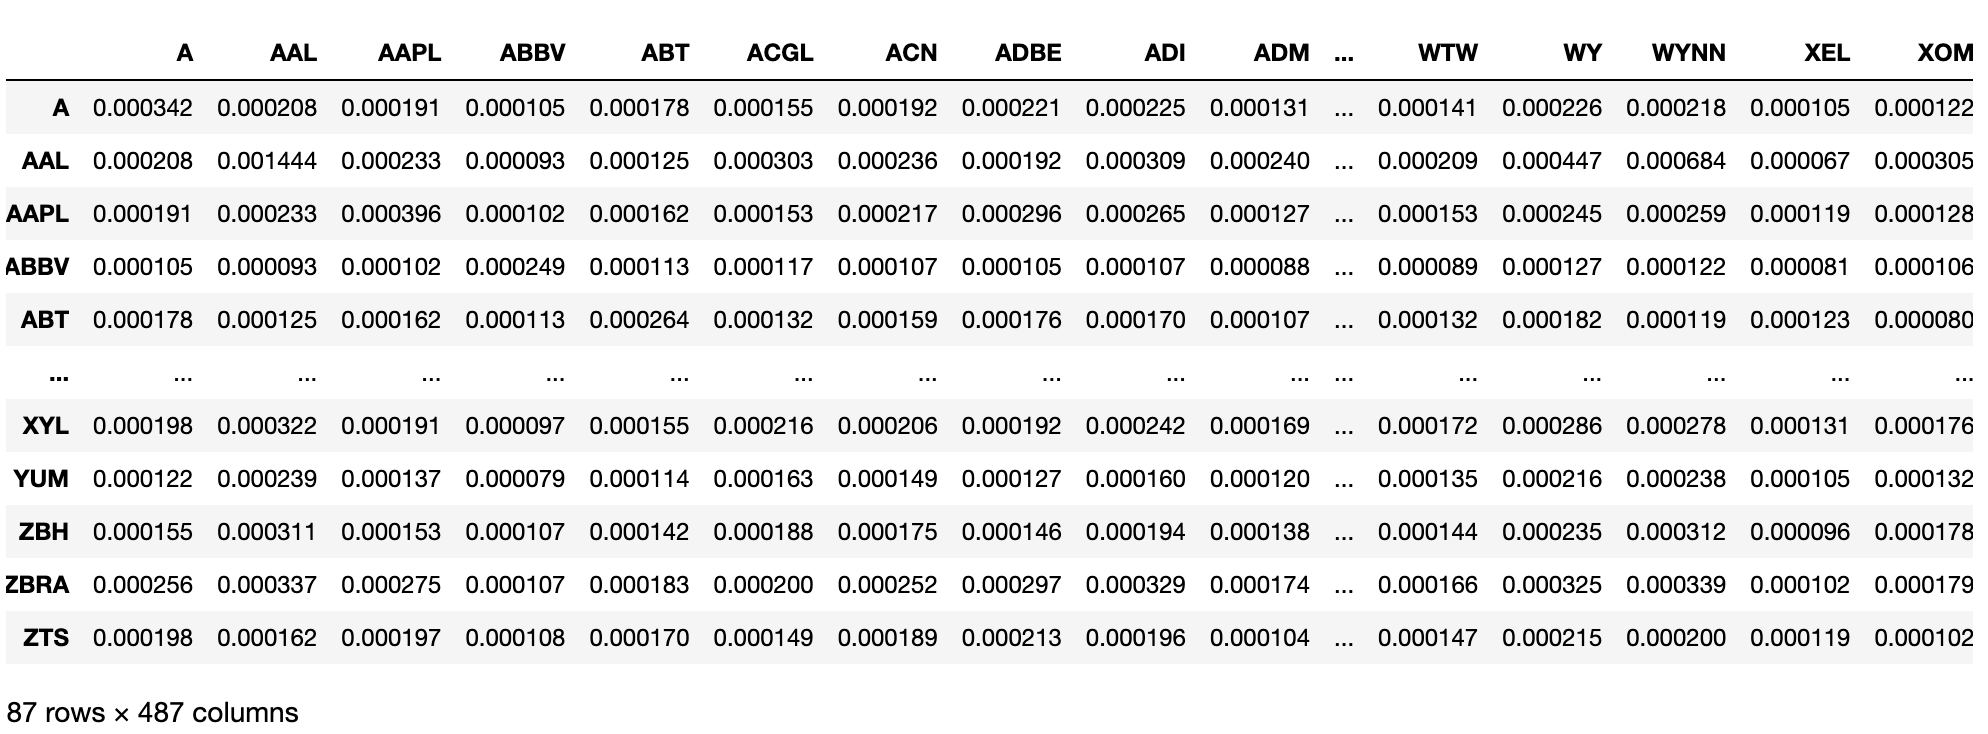
\includegraphics[scale = 0.3]{\pathtoimages/cov.png}
\end{figure}
Note: There are fewer than 500 columns because some of the current S\&P constituents weren't publicly traded companies in 2019.
\end{frame}

\section{Principal Component Analysis (PCA)}


\begin{frame}
\begin{center}
\Huge Principal Component Analysis (PCA)
\end{center}
\end{frame}


\begin{frame}
\frametitle{Eigenvectors and Eigenvalues}
From the spectral theorem, we know that $\Sigma$ is diagonalizable, since it is symmetric. If $\Sigma$ is $k\times k$, and the respective eigenvectors and eigenvalues are ${\boldsymbol v_1}, {\boldsymbol v_2},\ldots, {\boldsymbol v_k}$ and $\lambda_1, \lambda_2,\ldots, \lambda_k$. Then the total variance is $\lambda_1 + \lambda_2+\ldots+\lambda_k$, and the fraction of variance explained by eigenvector ${\boldsymbol v_i}$ is
$$
\frac{\lambda_i}{\lambda_1 +\lambda_2+\ldots+\lambda_i+\ldots+\lambda_k}.
$$
\end{frame}

\begin{frame}[t]
\frametitle{Eigenvectors and Eigenvalues Example}
\begin{Example}
Consider $\Sigma = \left(\begin{array}{c c} 1	&	0.5\\ 0.5 & 1\end{array}\right)$. Find the eigenvectors and eigenvalues.
\end{Example}

\end{frame}

\begin{frame}
\frametitle{Principal Component Analysis}
{\bf Principal component analysis (PCA)} is a dimension reduction technique. It explains some of the variance of the original data in terms of a few eigenvectors with the largest eigenvalues. 

\end{frame}

\begin{frame}
\frametitle{Principal Component Analysis Figure}

\begin{center}
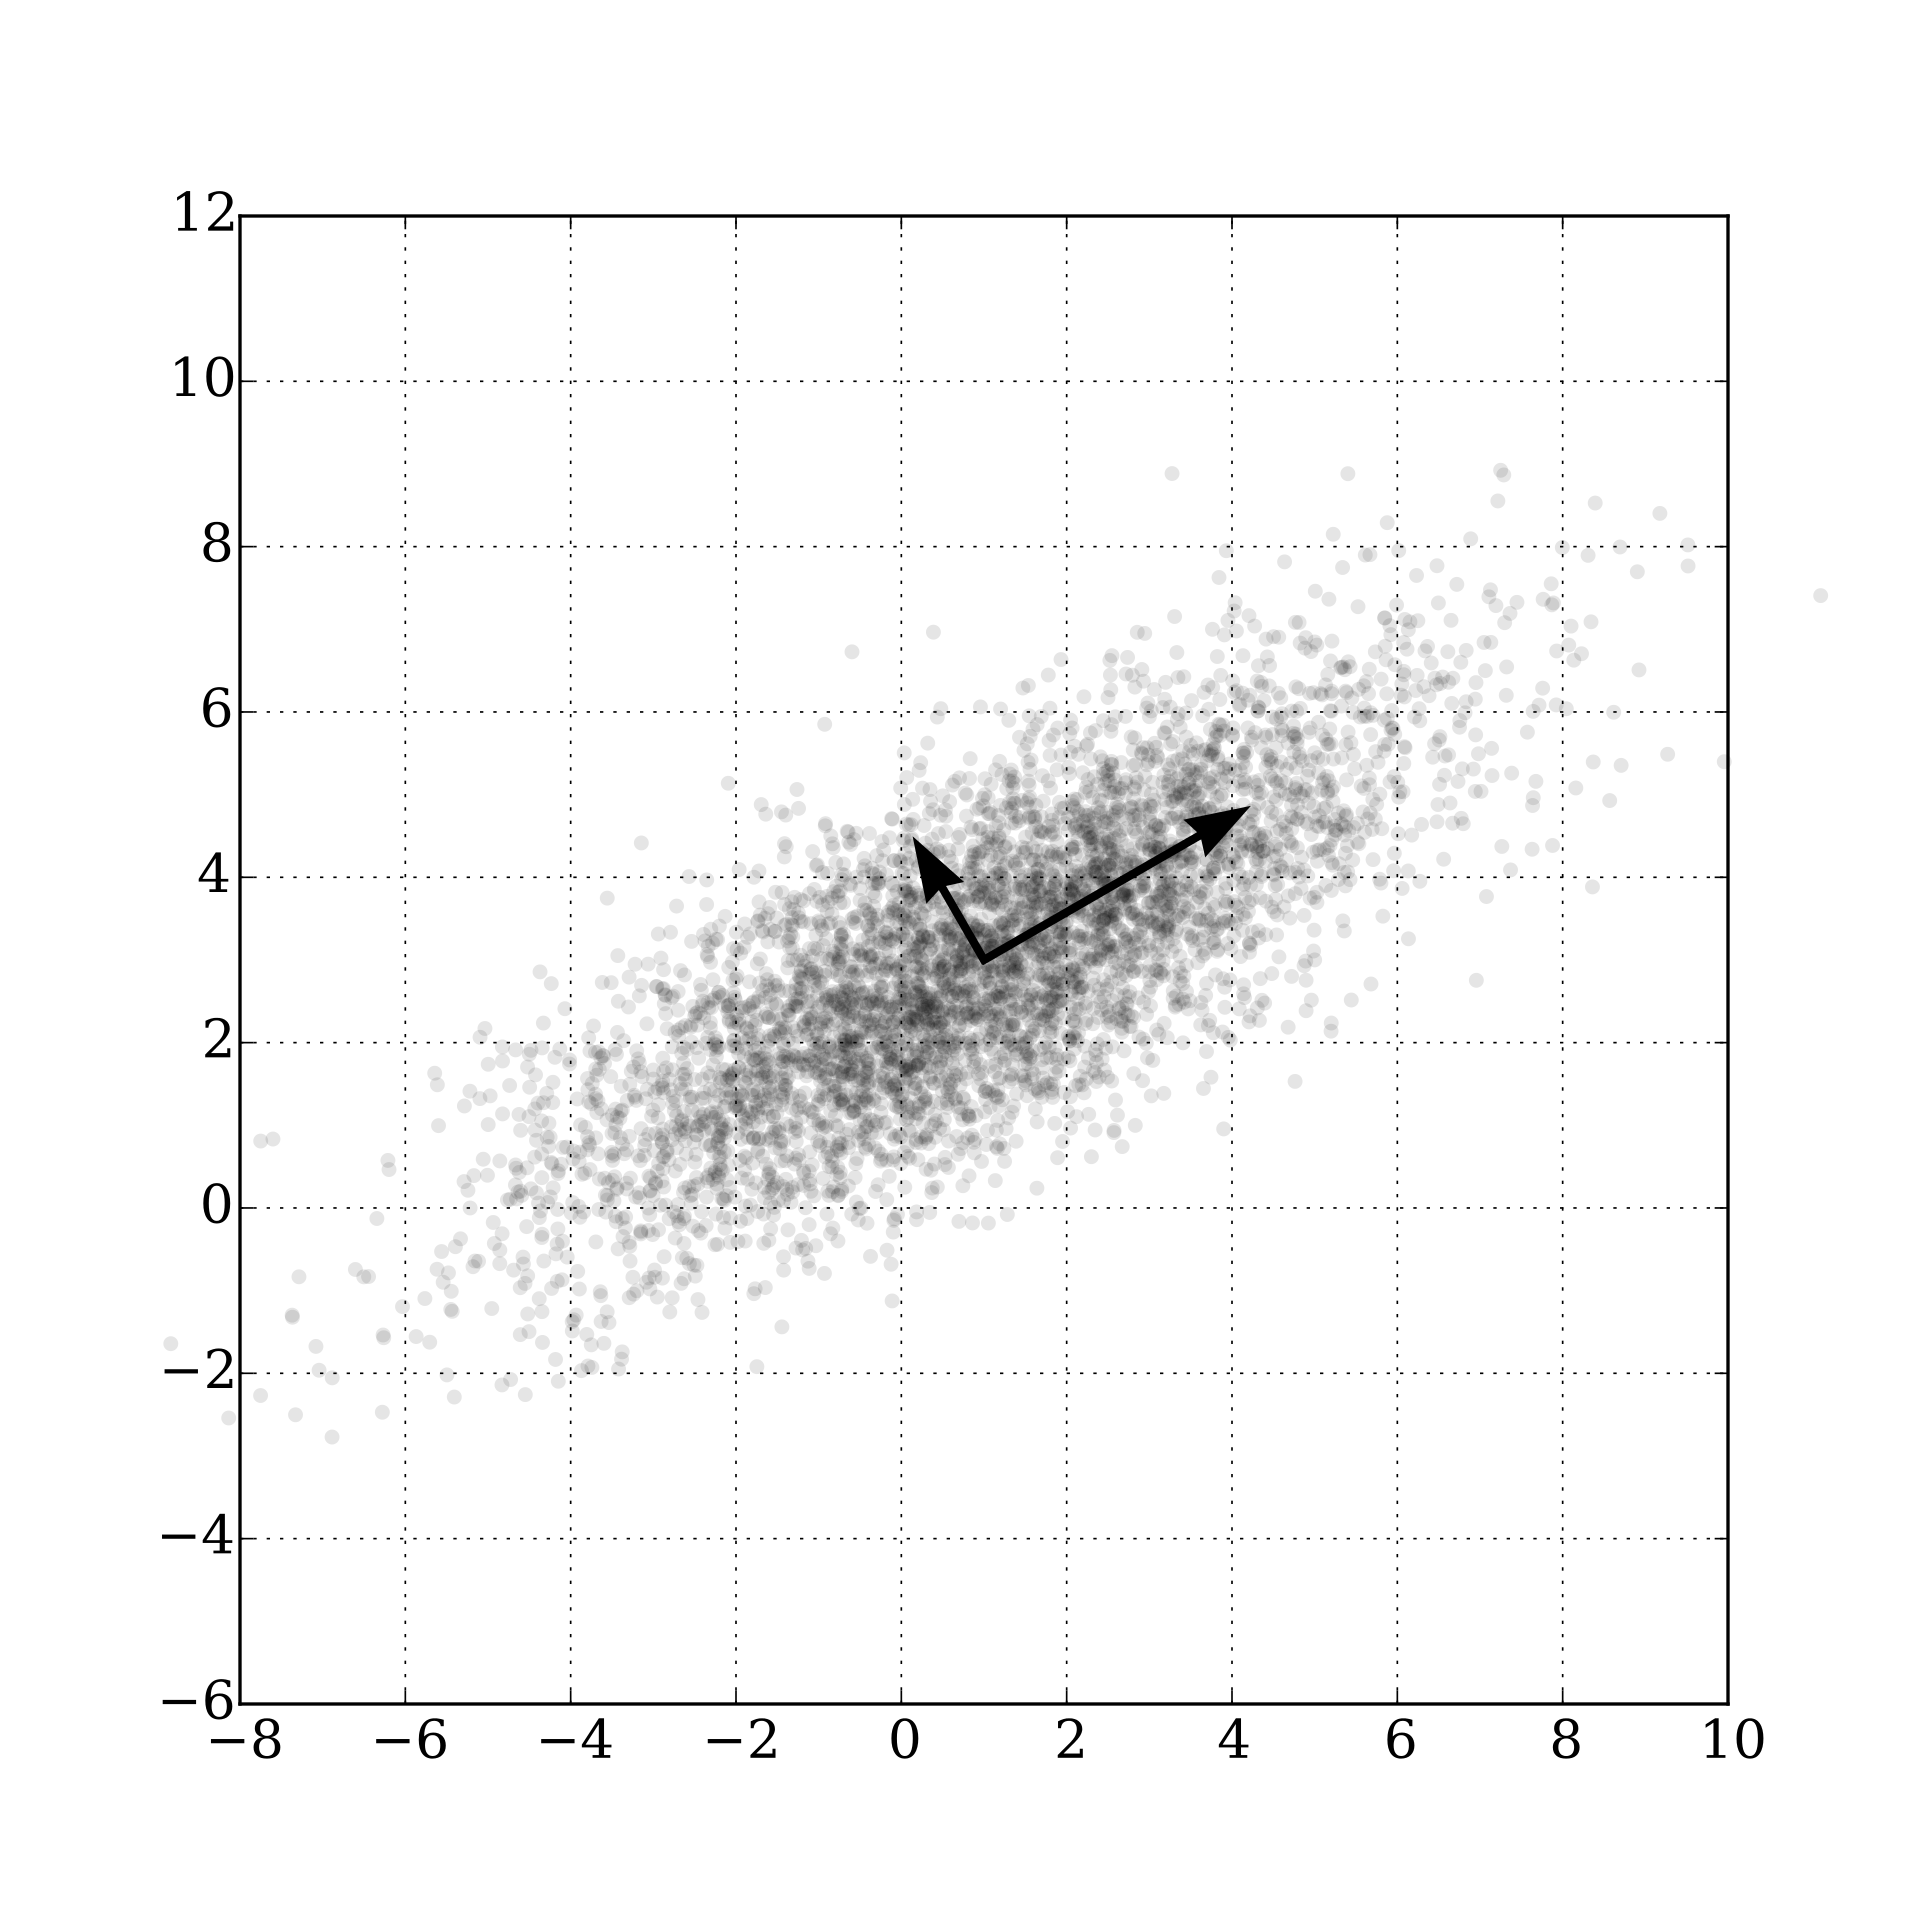
\includegraphics[scale = 0.1]{\pathtoimages/PCA_fig.png}
\end{center}
\end{frame}

\begin{frame}
\frametitle{Principal Component Analysis Steps}

\begin{enumerate}
\item[1.] Collect your data.
\item[2.] Standardize or demean your data.
\item[3.] Determine how much of the variance you need to explain or how many components are usable for your project.
\item[4.] Get the orthonormal basis of eigenvectors and eigenvalues.
\item[5.] Subset the orthonormal basis to the vectors corresponding to the largest $\ell$ eigenvalues, where the value of $\ell$ is based on step 3.
\item[6.] Calculate the ``loadings" of each observation on the remaining basis elements.
\end{enumerate}
\end{frame}

\begin{frame}
\frametitle{Convention}
Let's assume that 
$$
i < j\qquad\text{implies}\qquad \lambda_i \geq \lambda_j.
$$ 
In other words, we've rearrange our eigenvalues and corresponding eigenvectors so that the eigenvalues are in descending order.
\end{frame}

\begin{frame}
\frametitle{What are Loadings?}
\small
Suppose $\Sigma$'s eigenvectors are the orthonormal eigenbasis $({\boldsymbol v_1}, {\boldsymbol v_2},\ldots, {\boldsymbol v_k})$. Then observation ${\boldsymbol u}$ can be written as
$$
{\boldsymbol u} = \alpha_1 {\boldsymbol v_1} + \alpha_2 {\boldsymbol v_2} +\ldots + \alpha_\ell {\boldsymbol v_\ell}+ \ldots +\alpha_k {\boldsymbol v_k}\qquad\text{where}\qquad \alpha_i = \frac{{\boldsymbol u} \bullet {\boldsymbol v_i}}{\|{\boldsymbol v_i}\|^2} = {\boldsymbol u} \bullet {\boldsymbol v_i}.
$$
We say that ${\boldsymbol u}$ has a {\bf loading} of $\alpha_i$ on ${\boldsymbol v_i}$.

A good approximation of $\boldsymbol u$ is the first $\ell$ components. Therefore, we can think of $\boldsymbol u$ as more or less the same as
$$
\left(\begin{array}{c} \alpha_1\\ \alpha_2\\ \vdots\\ \alpha_\ell \end{array}\right)
$$
where the basis for this vector is $({\boldsymbol v_1}, {\boldsymbol v_2}, \ldots, {\boldsymbol v_\ell})$.

\end{frame}

\begin{frame}[fragile]
\frametitle{Principal Component Analysis Example}
\begin{Example}
Use PCA to represent the S\&P 500 constituent data from before on a two dimensional scatter plot.
\end{Example}
\begin{multicols}{2}
\begin{lstlisting}[language=Python]
import numpy as np
import matplotlib.pyplot as plt

# Use Seaborn style
plt.style.use('seaborn')

# S and data are as calculated previously

# Get the eigenvalues and eigenvectors
evals, evecs = np.linalg.eigh(S)

# Indices in descending order
idx = evals.argsort()[::-1]

# Change order
evecs, evals = evecs[idx], evals[idx]

# Convert the observations to a numpy array
X = data.values

# Get the mean of each firm's return
x_bar = X.mean(axis = 0)

# Demean X
X -= x_bar

# Calculate loadings using the dot product
loadings = X @ evecs[:, 0:2]

# Unpack results
x, y = zip(*loadings)

# Get scatter plot
plt.scatter(x, y)

# Create x- and y-abels
plt.xlabel('PCA1'); plt.ylabel('PCA2')

# Give the plot a title
plt.title(r'S\&P 500 Data with Dimension Reduction')

# Save the figure
plt.savefig(path + r'ex4-2.png')

plt.show()
\end{lstlisting}
\end{multicols}
\end{frame}

\begin{frame}
\frametitle{Principal Component Analysis Result}
\begin{figure}
\centering
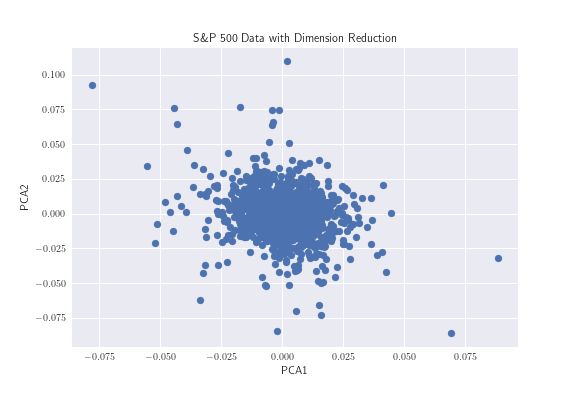
\includegraphics[scale = 0.4]{\pathtoimages/ex4-2.png}
\end{figure}

\end{frame}

\begin{frame}
\frametitle{Reconstruction}
If we have data with mean $ {\boldsymbol \mu}$, and we used the loadings of the first $\ell$ eigenvectors ${\boldsymbol v_1}, {\boldsymbol v_2},\ldots, {\boldsymbol v_\ell}$ to approximate ${\boldsymbol u}$, then this is making the assumption
$$
{\boldsymbol u} \approx  {\boldsymbol \mu} + \alpha_1 {\boldsymbol v_1} + \alpha_2 {\boldsymbol v_2}+\ldots + \alpha {\boldsymbol v_\ell},
$$
where $\alpha_i$ is the loading corresponding to ${\boldsymbol v_i}$. 

\end{frame}

\begin{frame}
\frametitle{Why Standardize?}
PCA results are affected by the scale of your data. However, in many applications scale is already known and users are more interested in correlations within the data. 
\end{frame}

\section{Clipping Covariance Matrices}

\begin{frame}
\begin{center}
\Huge Clipping Covariance Matrices
\end{center}
\end{frame}

\begin{frame}
\frametitle{Positive Definite Matrices}
Using the dot product, a matrix $S$ is {\it positive definite} if
$$
{\boldsymbol x^T }S {\boldsymbol x} > 0 \qquad\text{for all}\qquad {\boldsymbol x} \neq {\boldsymbol 0}.
$$
Since a covariance matrix is diagonalizable due to the spectral theorem, a covariance matrix will be positive definite if and only if all its eigenvalues are positive.
\end{frame}

\begin{frame}
\frametitle{Negative and Zero Eigenvalues}

\begin{itemize}
\item When $S$ is a covariance matrix, it never makes sense to have negative eigenvalues. These results are simply numerical errors.
\item A zero eigenvalue indicates one variable can be written as a linear combination of the others, which may or may not make sense given the context.
\end{itemize}

\end{frame}

\begin{frame}[fragile]
\frametitle{Negative and Zero Eigenvalues Example}
\begin{lstlisting}[language=Python]
# Import modules
import numpy as np
import matplotlib.pyplot as plt
from scipy.stats import norm

# Set the random seed
np.random.seed(0)

# Generate normal random variables
X = norm.rvs(size = (50, 100))

# Get the covariance matrix
S = np.cov(X, rowvar = False)

# Get the eigenvalues
evals, _ =  np.linalg.eigh(S)

print(f'The sample covariance matrix has {np.sum(np.isclose(evals, 0))}',
      r'eigenvalues numerically indistinguishable from 0.')
\end{lstlisting}

It says there are 51 eigenvalues numerically indistinguishable from 0. The true covariance matrix is the identity $I$ and therefore the only true eigenvalue is 1.
\end{frame}

\begin{frame}
\frametitle{Clip Covariance Matrices}

One solution is to ``clip" the sample covariance matrix. Simply replace all the eigenvalues that are too small with something bigger and reconstruct the covariance matrix.

\end{frame}

\begin{frame}[fragile]
\frametitle{Clip Covariance Matrices Example}
\small
Using the results from before. 
\begin{multicols}{2}
\begin{lstlisting}[language=Python]
# Get the standard deviations
stds = np.sqrt(np.diag(S))

# Get the correlation matrix
C = np.diag(1/stds) @ S @ np.diag(1/stds)

# Get the eigenvalues and vectors of C
evals_c, evecs_c = np.linalg.eigh(C)

# Make lam_min small positive outside of np.isclose threshold
lam_min = 1e-7

# Replace with smallest positive
evals_c[evals_c < lam_min] = lam_min

# Reconstruct correlation matrix
C_new = evecs_c @ np.diag(evals_c) @ evecs_c.T

# Make sure still correlation matrix
C_new = (np.diag(np.sqrt(1/np.diag(C_new))) @ C_new
            @ np.diag(np.sqrt(1/np.diag(C_new))))

# Multiply by standard deviations to make it covariance matrix
S_new = np.diag(stds) @ C_new @ np.diag(stds)

# Get the eigenvalues
evals_new, _ =  np.linalg.eigh(S_new)

print(f'The new covariance matrix has {np.sum(np.isclose(evals_new, 0))}',
      r'eigenvalues numerically indistinguishable from 0.')
\end{lstlisting}
\end{multicols}
Now it says all the eigenvalues are positive! Inspection shows that the covariance matrix estimate is otherwise very similar to the sample covariance matrix.
\end{frame}

\begin{frame}
\frametitle{Marchenko-Pastur Theorem}
\small
\begin{Theorem}
Consider a matrix of independent and identically distributed random observations $X$ of size $T\times N$, where the underlying process generating the observations has mean 0 and variance $\sigma^2$. If $q = T/N > 1$ is constant, the matrix $C = \frac{1}{T} X^T X$ has eigenvalues that converges to a distribution with probability density function
$$
f(\lambda) = \begin{cases} \frac{q}{2\pi\sigma^2} \frac{\sqrt{(\lambda_+ - \lambda)(\lambda - \lambda_-)}}{\lambda}, & \lambda_- \leq \lambda \leq \lambda_+\\ 0, & \text{otherwise}\end{cases}
$$
where
$$
\lambda_- = \sigma^2 \left(1 - \sqrt{\frac{1}{q}}\right)^2\qquad\text{and}\qquad \lambda_+ = \sigma^2 \left(1 + \sqrt{\frac{1}{q}}\right)^2.
$$
\end{Theorem}
\end{frame}

\begin{frame}[fragile]
\frametitle{Marchenko-Pastur Example}

\begin{lstlisting}[language=Python]
# Import modules
import numpy as np
import matplotlib.pyplot as plt
from scipy.stats import norm
import time

# Use LaTeX
plt.rcParams['text.usetex'] = True

# Use Seaborn style
plt.style.use('seaborn')

# Set the random seed
np.random.seed(0)

# Start the clock
start_time = time.perf_counter()

# Generate normal random variables
X = norm.rvs(size = (100_000, 10_000))

\end{lstlisting}
\end{frame}

\begin{frame}[fragile]
\frametitle{Marchenko-Pastur Example}

\begin{lstlisting}[language=Python]
# Get the number of observations and variables
T, N = X.shape

# Get correlation matrix
C = np.corrcoef(X, rowvar = False)

# q is the number of observations divided by the number of variables
q = T/N

# Get eigenvalues
evals, _ = np.linalg.eigh(C)

# Get support of Marchenko–Pastur distribution
lam_minus, lam_plus = (1 - np.sqrt(1/q))**2, (1 + np.sqrt(1/q))**2 
        
# Define pdf
def f(lam):
    
    # Support of Marchenko–Pastur distribution
    if lam_minus <= lam <= lam_plus:
    
        return q/(2 * np.pi) * np.sqrt((lam_plus - lam) * (lam - lam_minus))/lam
                
    else:
        
        return 0

\end{lstlisting}
\end{frame}



\begin{frame}[fragile]
\frametitle{Marchenko-Pastur Example Cont.}

\begin{lstlisting}[language=Python]

# Get lam_vals
lam_vals = np.linspace(lam_minus, lam_plus, 100)

# Get density values
f_vals = [f(lam) for lam in lam_vals]

# Plot histogram
plt.hist(evals, density = True, bins = int(np.sqrt(N)), label = 'Simulated Distribution')

# Plot density
plt.plot(lam_vals, f_vals, label = 'Density')

# Add legend
plt.legend()

# Add x-label
plt.xlabel(r'$\lambda$')

# Add y-label
plt.ylabel(r'Density')

# Add title to plot
plt.title(r'Marchenko–Pastur Distribution')

# Save the figure
plt.savefig(path + r'ex4-3.png')

plt.show()

print(f'This script took {(time.perf_counter() - start_time)/60:.2f} minutes to run.')
\end{lstlisting}

\end{frame}

\begin{frame}[fragile]
\frametitle{Marchenko-Pastur Result}

\begin{center}
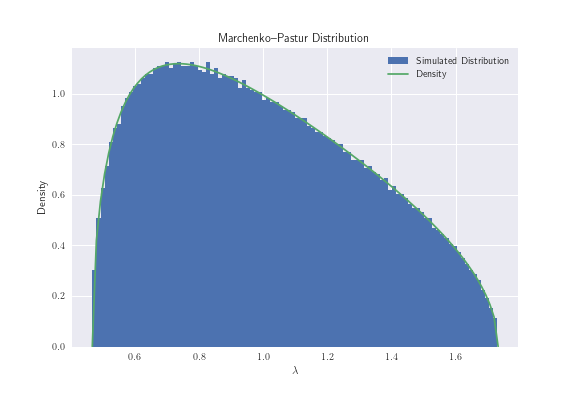
\includegraphics[scale = 0.5]{\pathtoimages/ex4-3.png}
\end{center}

\end{frame}

\begin{frame}
\frametitle{How to use it?}
Consider eigenvalue $\lambda$ of the covariance matrix.
\begin{itemize}
\item If $\lambda > \lambda_+$, then result consistent with signal. 
\item If $\lambda \leq \lambda_+$, the result is probably just random noise. Replace values less than $\lambda_+$ with mean of values less than $\lambda_+$.
\end{itemize}

\end{frame}

\begin{frame}[fragile]
\frametitle{S\&P 500 Constituent Example}
Suppose we have the S\&P 500 constituent data from before.
\begin{lstlisting}[language=Python]
# Get the standard deviations
stds = np.sqrt(np.diag(S))

# Calculate correlation matrix
C = np.diag(1/stds) @ S @ np.diag(1/stds)

# Get the eigenvalues and vectors
evals, evecs =  np.linalg.eigh(C)

# Save q
q = data.shape[0]/data.shape[1]

# Get support of Marchenko-Pastur distribution
lam_minus, lam_plus = (1 - np.sqrt(1/q))**2, (1 + np.sqrt(1/q))**2 
        
# Define pdf
def f(lam):
    
    # Support of Marchenko–Pastur distribution
    if lam_minus <= lam <= lam_plus:  
        return q/(2 * np.pi) * np.sqrt((lam_plus - lam) * (lam - lam_minus))/lam                
    else:       
        return 0
    
# Get lam_vals
lam_vals = np.linspace(lam_minus, lam_plus, 100)

# Get density values
f_vals = [f(lam) for lam in lam_vals]
\end{lstlisting}
\end{frame}


\begin{frame}[fragile]
\frametitle{S\&P 500 Constituent Example}
\begin{lstlisting}[language=Python]
# Plot histogram
plt.scatter(evals[evals > lam_plus], np.zeros(np.sum(evals > lam_plus)), 
            label = 'Signal Eigenvalues')

plt.scatter(evals[evals <= lam_plus], np.zeros(np.sum(evals <= lam_plus)), 
            label = 'Noise Eigenvalues', color = 'gray')

# Plot density
plt.plot(lam_vals, f_vals, label = 'Density', color = 'green')

# There are 3 eigenvalues much larger than 10
plt.xlim([0, 10])

# Add legend
plt.legend()

# Add x-label
plt.xlabel(r'$\lambda$')

# Add y-label
plt.ylabel(r'Density')

# Add title to plot
plt.title(r'S\&P 500 Constituents')

# Save the figure
plt.savefig(path + r'ex4-4.png')

plt.show()
\end{lstlisting}
\end{frame}

\begin{frame}[fragile]
\frametitle{S\&P 500 Constituent Example}
Only the values past $\lambda_+$ are consistent with signal. There are three eigenvalues greater than 10 which are not shown.
\begin{figure}
\centering
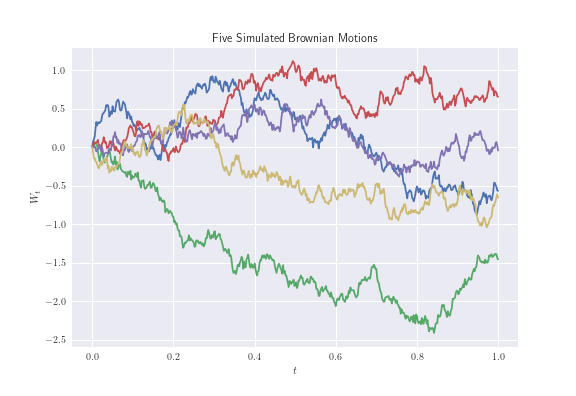
\includegraphics[scale = 0.4]{\pathtoimages/ex4-4.png}
\end{figure}

\end{frame}


\begin{frame}[fragile]
\frametitle{Clip Matrix}
\begin{lstlisting}[language=Python]
# Initialize new eigenvalues
evals_new = evals

# Replace noise eigenvalues with mean
evals_new[evals_new < lam_plus] = np.mean(evals_new[evals_new < lam_plus])

# Construct new correlation matrix
C_new = evecs @ np.diag(evals_new) @ evecs.T

# Make sure still correlation matrix
C_new = np.diag(1/np.sqrt(np.diag(C_new))) @ C_new @ np.diag(1/np.sqrt(np.diag(C_new)))

# Make new covariance matrix
S_new = np.diag(stds) @ C_new @ np.diag(stds)
\end{lstlisting}
\end{frame}

\begin{frame}
\frametitle{$\epsilon$-$\delta$ Limit Definition on YouTube}
Check out Marcos Lopez de Prado's talk. He covers covariance clipping and the Marchenko–Pastur distribution near the beginning  {\tiny(\url{https://www.youtube.com/watch?v=tODXAJDZtow})}.
\begin{center}

\includegraphics[scale = 0.30]{\pathtoimages/lopez_de_prado.png}
\end{center}
\end{frame}

\section{Stochastic Calculus} 

\begin{frame}
\begin{center}
\Huge Stochastic Calculus
\end{center}
\end{frame}

\subsection{Introduction} 

\begin{frame}
\frametitle{Source} 
I'm following these notes very closely: \url{http://www.columbia.edu/~mh2078/FoundationsFE/IntroStochCalc.pdf}
\end{frame}

\begin{frame}
\frametitle{Probability Triple}
We assume we have the probability space $(\Omega, \mathcal{F}, P)$ where
\begin{itemize}
\item $\Omega$ is the universe of possible outcomes.
\item $\mathcal{F}$ represents the $\sigma$-algebra of events in $\Omega$.
\item $P$ is the ``true" or physical probability measure.
\end{itemize}
\end{frame}

\begin{frame}
\frametitle{Filtration}
There is also a {\bf filtration} $\{\mathcal{F}_t\}_{t\geq 0}$ of $\sigma$-algebras that models the evolution of information through time. Since information increases over time $\mathcal{F}_s \subseteq \mathcal{F}_t$ for $s < t$.

If it is know by time $t$ whether or not an event $E$ has occurred, then we have $E\in\mathcal{F}_t$. If we are working with a finite horizon $[0, T]$, then we can take $\mathcal{F} = \mathcal{F}_T$.
\end{frame}

\begin{frame}
\frametitle{Stochastic Process}

\begin{Definition}
For a given probability space $(\Omega, \mathcal{F}, P)$, a {\bf stochastic process} is a collection of random variables indexed by $\mathcal{T}$. We often write $\{X_t | t \in\mathcal{T}\}$ to denote a stochastic process, and we think of $\mathcal{T}$ as the time index.
\end{Definition}
\end{frame}

\begin{frame}
\frametitle{Stochastic Process Example}

\begin{Example}
For a high yield bond portfolio, we can model the total number of defaulted bonds this year up to day $t$ as a stochastic process. Denote the number of defaulted bonds on day $t$ by $N_t$. In this case, $\mathcal{T} = \{1, 2, 3,\ldots, 252\}$, assuming there are 252 days when the market is open. Using our prior notation, the stochastic process is $\{N_t | t\in\mathcal{T}\}$.
\end{Example}

\end{frame}

\begin{frame}

\frametitle{$\mathcal{F}_t$-Adapted}
\begin{Definition}
We say that a stochastic process $X_t$ is $\mathcal{F}_t${\bf-adapted} if for every $t$ in $\mathcal{T}$ the information about $X_t$ is contained in $\mathcal{F}_t$.
\end{Definition}
\end{frame}

\begin{frame}
\frametitle{Brownian Motion}
\begin{Definition}
A stochastic process $\{W_t | t\geq 0\}$ is a {\bf standard Brownian motion} if the following hold.
\medskip

\begin{quote}
\begin{enumerate}
\item[BM.1] $W_0 = 0$.
\item[BM.2] It has continuous sample paths.
\item[BM.3] $W_{t_1} - W_{s_1}$ and $W_{t_2} - W_{s_2}$ are independent for $0\leq s_1 \leq t_1 \leq s_2 \leq t_2$.
\item[BM.4] $W_t - W_s \sim{\mathcal{N}(0, t - s)}$ for $0\leq s \leq t$.
\end{enumerate}
\end{quote}
\end{Definition}
\end{frame}

\begin{frame}
\frametitle{Simulating Brownian Motion}
Suppose that we want to simulate a Brownian motion on the interval $[0, T]$. Then construct a partition of the interval
$$
0 = t_0 < t_1 <\ldots < t_{n - 1} < t_n = T.
$$
For $i = 1, 2,\ldots, n$, generate $Z_i\sim{\mathcal{N}(0, 1^2)}$. Then 
$$
\widetilde{W}_{t_k} = \begin{cases} 0	,	&	k = 0\\
						\sum_{i = 1}^k Z_i \sqrt{\Delta t_i},	&	k = 1, 2,\ldots, n
						\end{cases}
$$
is ``approximately" Brownian motion.
\end{frame}

\begin{frame}[fragile]
\frametitle{Python Code: Five Brownian Motions on [0, 1]}

\begin{multicols}{2}
\begin{lstlisting}[language=Python]
import numpy as np, matplotlib.pyplot as plt
from scipy.stats import norm

# Use LaTeX
plt.rcParams['text.usetex'] = True

# Use Seaborn style
plt.style.use('seaborn')

# Set the random seed
np.random.seed(0)

# Break up into n discrete intervals
n = 500

# Simulate five Brownian motions
for _ in range(5):
    
    # Simulate Brownian motion for t in [0, 1]
    Z = norm.rvs(scale = np.sqrt(1/n), size = n)
    
    # Take the cumulative sum; add 0 for the t = 0 value
    W = np.insert(np.cumsum(Z), 0, 0)
    
    # Plot results
    plt.plot(np.linspace(0, 1, n + 1), W)
    
# Add x-label
plt.xlabel(r'$t$')

# Add y-label
plt.ylabel(r'$W_t$')

# Add title to plot
plt.title(r'Five Simulated Brownian Motions')

# Save the figure
plt.savefig(path + r'ex4-5.png')

plt.show()
\end{lstlisting}
\end{multicols}
\end{frame}

\begin{frame}
\frametitle{Output}
Five Brownian motions on the interval $[0, 1]$, using a uniform partition that breaks $[0, 1]$ into 500 subintervals. 
\begin{center}
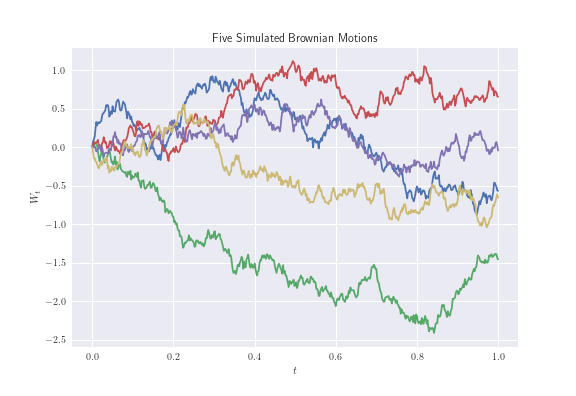
\includegraphics[scale = 0.4]{\pathtoimages/ex4-5.png}
\end{center}

\end{frame}


\begin{frame}
\frametitle{Martingale} 

\begin{Definition}
A stochastic process $\{X_t | 0\leq t \leq\infty\}$ is a {\bf martingale} with respect to the filtration $\mathcal{F}_t$ if the following hold.
\medskip

\begin{quote}
\begin{enumerate}
\item[M.1] $E\left[|X_t|\right] <\infty$ for all $t\geq 0$.
\item[M.2] $E\left[ X_{t + s} | \mathcal{F}_t\right] = X_t$ for all $t, s \geq 0$.
\end{enumerate}
\end{quote}
\end{Definition}

\end{frame}

\begin{frame}[t]
\frametitle{Martingale Example} 
\begin{Example}
Prove the following are martingales.
\begin{itemize}
\item[(a)] $W_t$
\item[(b)] $W_t^2 - t$
\item[(c)] $\exp\left(\theta W_t - \frac{\theta^2 t}{2}\right)$
\end{itemize}
\end{Example}

\end{frame}

\subsection{Quadratic Variation}

\begin{frame}
\frametitle{Quadratic Variation}
\begin{Definition}
Let $X_t$ be some stochastic process. The {\bf quadratic variation} of a stochastic process $X_t$ is
$$
\lim_{\|\mathcal{P}\|\to 0} \sum_{k = 1}^n \Big(X_{t_k} - X_{t_{k - 1}}\Big)^2,
$$
where $\mathcal{P}$ is an arbitrary partition of $[0, T]$ and $\|\mathcal{P}\| = \max\limits_k\{\Delta t_k\}$ is the mesh of the partition.
\end{Definition}
\end{frame}

\begin{frame}[t]
\frametitle{Quadratic Variation Example}
\begin{Example}
Compute the quadratic variation of the deterministic process $X_t = t^2$.
\end{Example}

\end{frame}

\begin{frame}
\frametitle{Quadratic Variation Differentiable Function}
Any differentiable function will end up having quadratic variance 0, like we saw for $t^2$ in our example. 
\end{frame}

\begin{frame}
\frametitle{Quadratic Variation of Brownian Motion}

\begin{Theorem}
The quadratic variation of a standard Brownian motion is equal to $T$ with probability 1.
\end{Theorem}

\begin{Theorem}[Levey's Theorem]
 A continuous martingale is a standard Brownian motion if and only if its quadratic variation over each interval $[0, t]$ is equal to $t$.
\end{Theorem}

\end{frame}

\begin{frame}[fragile]
\frametitle{Approximate Quadratic Variation Python Code}

\begin{lstlisting}[language=Python]
import numpy as np, matplotlib.pyplot as plt
from scipy.stats import norm

# Use LaTeX
plt.rcParams['text.usetex'] = True

# Use Seaborn style
plt.style.use('seaborn')

# Set the random seed
np.random.seed(0)

# Define n-values
n_vals = [10, 100, 1000, 10000]

# Set up subplots
fig, ax = plt.subplots(2, 2, sharey = True, figsize = (15, 10), dpi = 125)

# Simulate five Brownian motions
for i, n in enumerate(n_vals):
    
    # Get row and column
    row, col = i//2, i % 2
    
    # Difference of two Brownian motions is normal
    dW = norm.rvs(scale = np.sqrt(1/n), size = (3, n))
    
    # Calculate quadratic variance
    quad_var = np.cumsum(dW**2, axis = 1)

\end{lstlisting}
\end{frame}

\begin{frame}[fragile]
\frametitle{Approximate Quadratic Variation Python Code}

\begin{lstlisting}[language=Python]    
    # Plot results
    for j in range(3):
        
        ax[row, col].plot(np.linspace(1/n, 1, n), quad_var[j, :])

    # Plot t
    ax[row, col].plot(np.linspace(1/n, 1, n), np.linspace(1/n, 1, n), 
         label = r'$t$')
    
    # Add x-label
    ax[row, col].set_xlabel(r'$t$')

    # Add y-label
    ax[row, col].set_ylabel(r'$\displaystyle\sum_{k = 1}^{n} (W_{t_k} - W_{t_{k - 1}})^2$')
    
    # Give plot a title
    ax[row, col].set_title(f'$n$ = {n}')
    
    # Add legend
    ax[row, col].legend()

# Add title to plot
plt.suptitle(r'Approximate Quadratic Variation')

# Save the figure
plt.savefig(path + r'ex4-6.png')

plt.show()
\end{lstlisting}
\end{frame}

\begin{frame}[fragile]
\frametitle{Approximate Quadratic Variation Result}
From the four subplots, we see that $\lim\limits_{n\to\infty} \sum_{k = 1}^n \left(W_{t_k} - W_{t_{k - 1}}\right)^2 = T$.
\begin{figure}
\centering
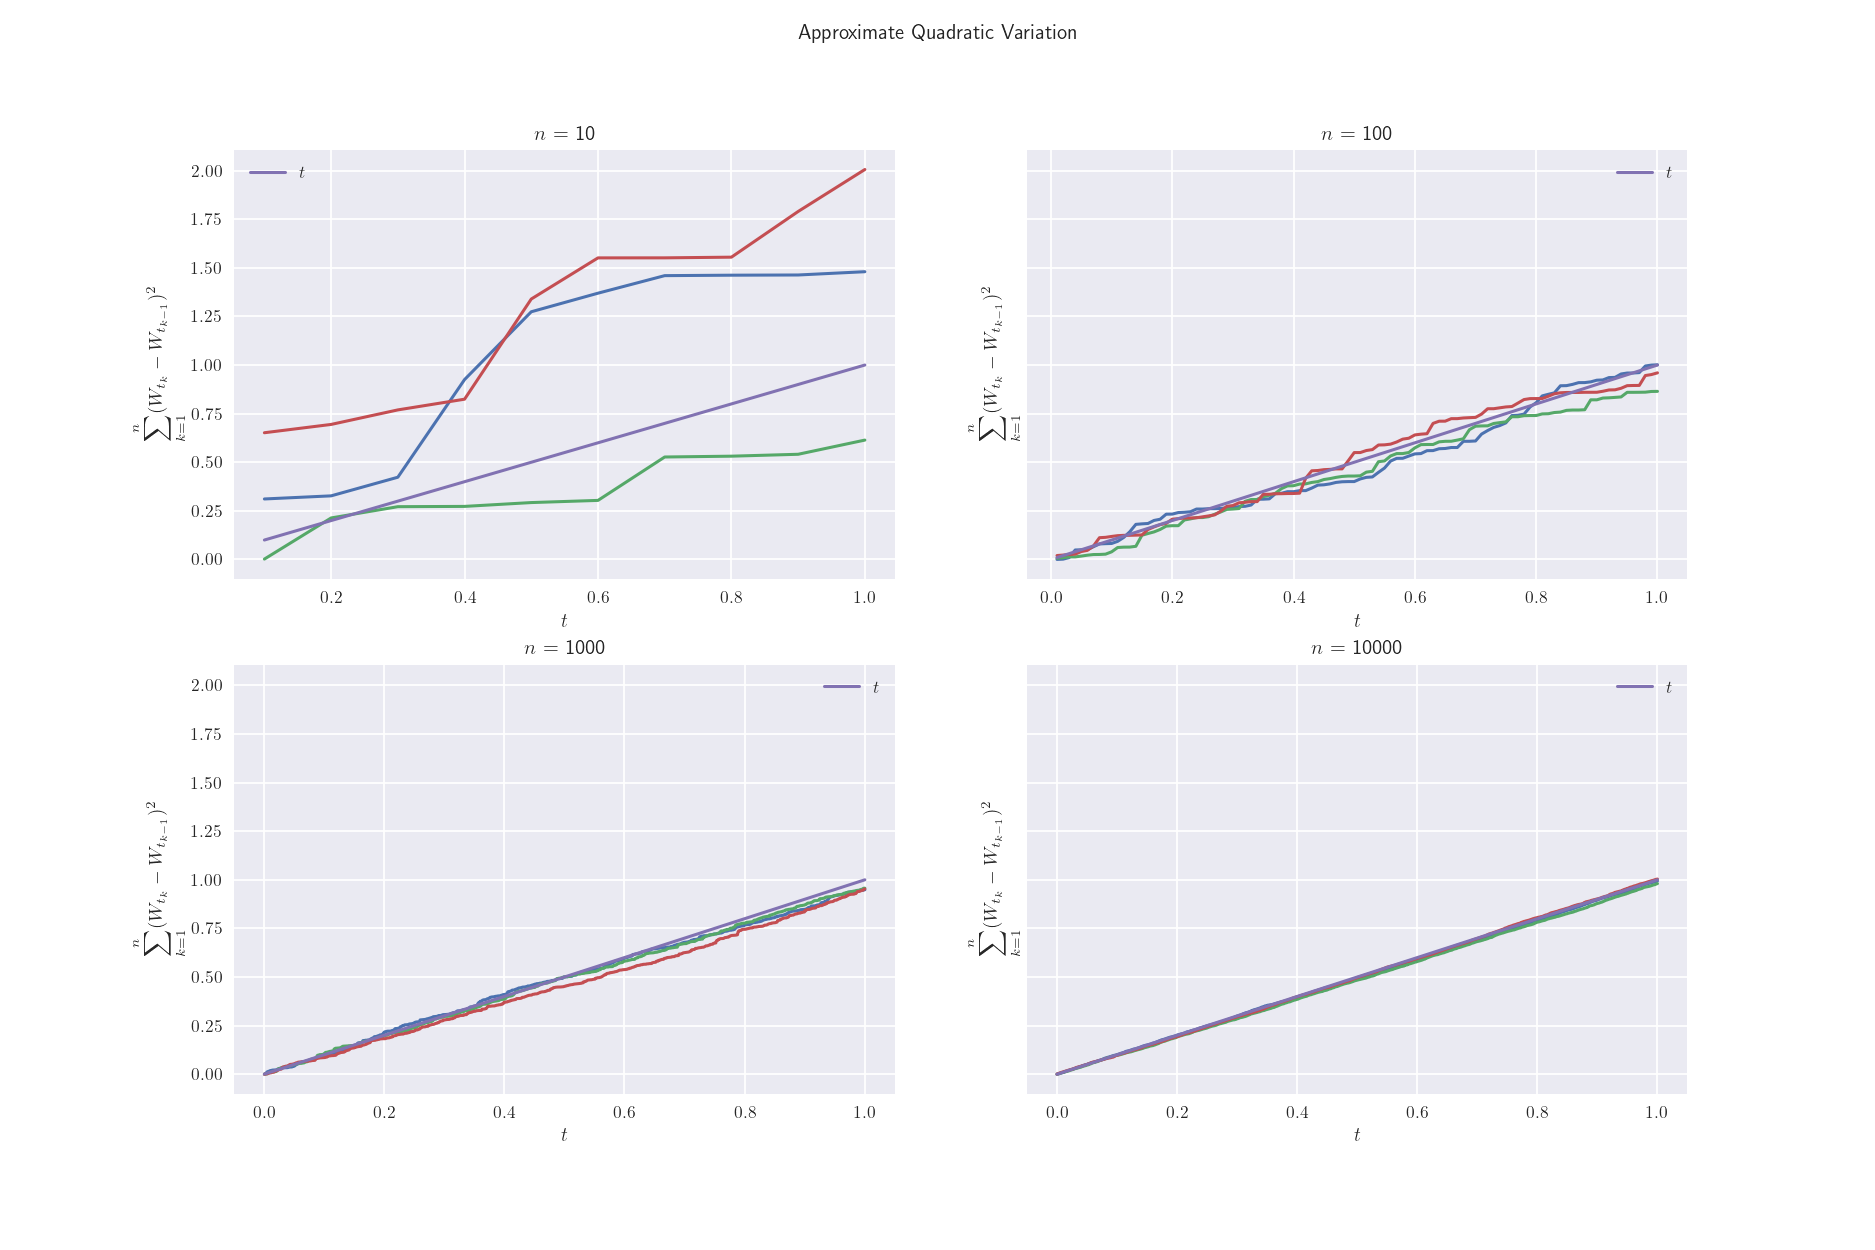
\includegraphics[scale = 0.25]{\pathtoimages/ex4-6.png}
\end{figure}
\end{frame}



\subsection{It\^o Integrals}

\begin{frame}
\frametitle{It\^o Integrals}
\begin{Definition}
The {\bf It\^o Integral} of $X_t$ with respect to standard Brownian motion
$$
\int_0^T X_t\ dW_t = \lim_{\| P\|\to 0} \sum_{k = 1}^{n } X_{t_{k - 1}} (W_{t_k} - W_{t_{k - 1}}),
$$
where $\mathcal{P} = (t_0, t_1,\ldots, t_n)$ is an arbitrary partition.
\end{Definition}

\end{frame}

\begin{frame}
\frametitle{It\^o Integrals Example}
\small 
\begin{Example}
Assuming the It\^o integral exists, compute $\int_0^T W_t\ dW_t$.
\end{Example}

{\bf Solution.}
Consider the uniform partition $\Delta t = T/n$ and $t_k = k \Delta t$. Then
\begin{align*}
\int_0^ T W_t\ dW_t 	&= \lim_{n\to\infty}\sum_{k = 1}^n W_{t_{k - 1}} \left(W_{t_k} - W_{t_{k - 1}}\right)\\
				&= \lim_{n\to\infty}\frac{1}{2} \sum_{k = 1}^n \left[ W_{t_k}^2 - W_{t_{k - 1}}^2 - (W_{t_k} - W_{t_{k - 1}})^2\right]\\
				&=  \frac{1}{2} (W_{T}^2 - W_0^2) - \frac{1}{2}\lim_{n\to\infty} \sum_{k = 1}^n (W_{t_k} - W_{t_{k - 1}})^2\\
				&= \frac{1}{2} (W_{T}^2 - W_0^2) - \frac{1}{2}T\\
				&= \frac{1}{2} W_{T}^2 - \frac{1}{2}T.
\end{align*}

\end{frame}

\begin{frame}
\frametitle{Law of Iterated Expectations}
Suppose that $s \leq t \leq T$. Then
$$
E[X_T |\mathcal{F}_s] = E\Big[E[X_T|\mathcal{F}_t] \Big|\mathcal{F}_s\Big].
$$
Instead of writing $E[X_T |\mathcal{F}_t]$ we often write $E_t[X_T]$. Using this notation, the Law of Iterated Expectations is
$$
E_s[X_T] = E_s\Big[E_t[X_T]\Big].
$$
\end{frame}

\begin{frame}
\frametitle{It\^o Isometry}
\begin{Theorem}[It\^o Isometry]
We have
$$
E\left[\left(\int_0^T X_t\ dW_t\right)^2\right] = E\left[\int_0^T X_t^2\ dt\right]
$$
whenever
$$
E\left[\int_0^T X_t^2\ dt\right] < \infty.
$$
\end{Theorem}
\end{frame}



\end{document}
